% !TEX root = ./notes.tex
\chapter{Convection}\label{s.convection}

Hot air rises, as a glider pilot or hawk can tell you. The fluid velocities in question are very subsonic, so we have hydrostatic equilibrium to excellent approximation. But the fluid motions make an enormous difference for heat transport! This state of fluid motions induced by a temperature gradient is known as \emph{convection}. You can perform the following demonstration of the onset of convection.  Brew tea, and pour the hot tea into a saucepan that is on an unlit burner.  Use a straw with your thumb over the top to insert a layer of cold milk under the warm tea in the saucepan.  The temperature difference between the tea and milk will inhibit their mixing. Light the burner, and watch for the development of convection---you will know it when you see it.

\begin{figure}[htbp]
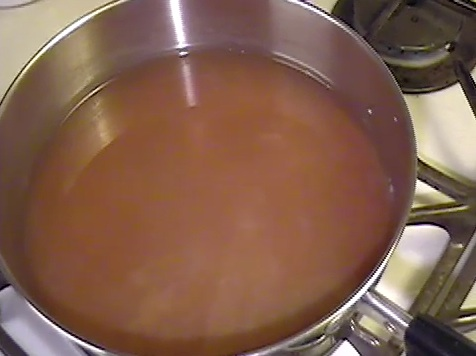
\includegraphics[width=180pt]{Figures/convection-1}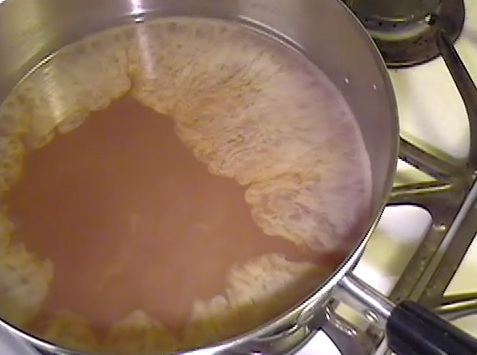
\includegraphics[width=180pt]{Figures/convection-2}
\caption{Onset of convection in a tea-milk mixture.\label{f.tea}}
\end{figure}

\section{Criteria for onset of convection}\label{s.convection-onset}

To understand this process, let's consider a fluid in planar geometry and hydrostatic equilibrium,
\begin{equation}
\frac{\dif P}{\dif r} = -\rho g.
\end{equation}
Now, imagine moving a blob of fluid upwards from $r$ to $r+h$.  We move the blob slowly enough that it is in hydrostatic equilibrium with its new surroundings, $P_{b}(r+h) = P(r+h)$, where the subscript $b$ refers to ``blob.'' We do move the blob quickly enough, however,  that it does not remain in \emph{thermal} equilibrium with its surroundings; that is, we move the blob \emph{adiabatically}.  The entropy of the blob is therefore constant, 
$S_{b}(r+h) = S_{b}(r) = S(r)$, and is therefore not, in general, equal to the entropy of the surrounding gas at $r+h$: $S_{b}(r+h)  \neq S(r+h)$.  

As the blob rises, it displaces some of the surrounding fluid. Archimedes tells us that if the displaced fluid is less massive than the blob, then the blob will sink.  We can rephrase this in terms of the volume occupied by a unit mass of fluid $V$: if the volume occupied by the blob is less than the volume of an equal mass of background, then the blob will sink. Translating this into an equation: if
\begin{eqnarray}
\lefteqn{V[P(r+h),S(r+h)] - V_{b}[P_{b}(r+h),S_{b}(r+h)] =}\nonumber\\
&&  V[P(r+h),S(r+h)] - V[P(r+h),S(r)] > 0
\label{e.archimedes}
\end{eqnarray}
then the blob will sink. If condition (\ref{e.archimedes}) is violated, the blob will continue to rise, and the system is unstable to convection.  
Figure~\ref{f.convective-schematic} has a cartoon of this process.

\begin{figure}[htbp]
\centerline{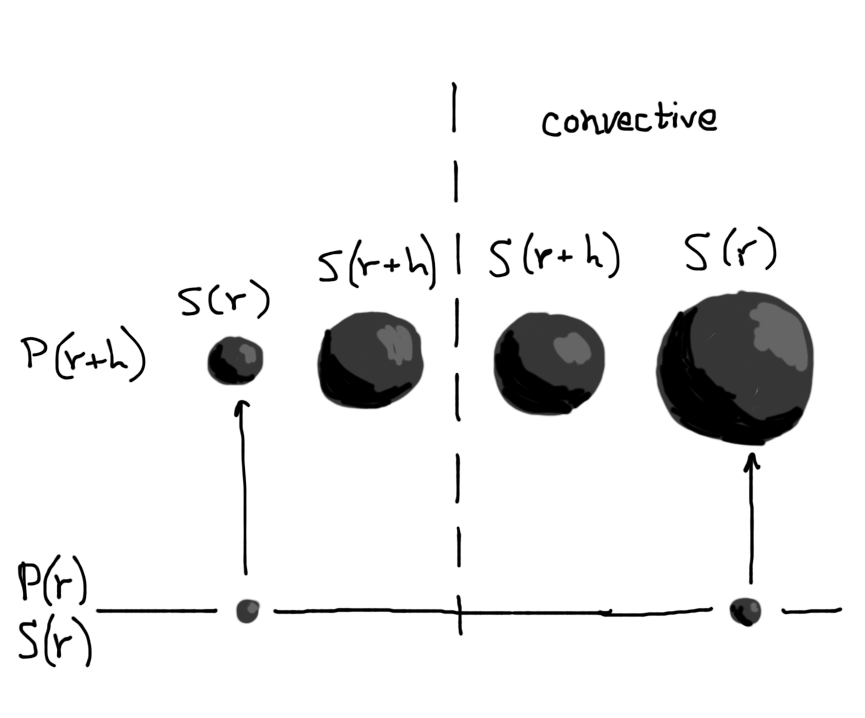
\includegraphics[width=\textwidth]{Figures/convective.png}}
\caption{\label{f.convective-schematic}Illustration of criteria for convective instability.  On the left, raising a blob a distance $h$ adiabatically and in pressure balance with its surrounding results in a higher density $V_{b} < V$.  This is stable: the blob will sink back.  On the right, the blob is less dense and hence buoyant: it will continue to rise.}
\end{figure}

Taking $h$ to be an infinitesimal displacement and expanding the left-hand side of equation~(\ref{e.archimedes}) gives us a local condition for stability:
\begin{equation}\label{e.convective-stability}
V[P(r+h),S(r)] + \tderiv{V}{S}{P}\frac{\dif S}{\dif r} - V[P(r+h),S(r)]  = \tderiv{V}{S}{P}\frac{\dif S}{\dif r} > 0 .
\end{equation}
Noting that
\begin{eqnarray*}
\tderiv{V}{T}{P} &=& \tderiv{V}{S}{P}\tderiv{S}{T}{P}\\
 &=& \frac{C_{P}}{T}\tderiv{V}{S}{P},
 \end{eqnarray*}
 we can rewrite equation~(\ref{e.convective-stability}) as
 \[
 \frac{T}{C_{P}}\tderiv{V}{T}{P}\frac{\dif S}{\dif r} > 0.
 \]
Now, $(\partial V/\partial T)_{P}$ is positive (gas expands on being heated), so our condition for stability is simply
 \begin{equation}\label{e.entropy-condition}
\frac{\dif S}{\dif r} > 0.
\end{equation}
In a convectively stable star, the entropy must increase with radius. if $\dif S/\dif r < 0$, then convection occurs and carries high-entropy material outward, where it will eventually mix with the ambient medium.  As a result, convection drives the entropy gradient toward the marginally stable configuration $\dif S/\dif r = 0$.  If a star is fully convective and mixes efficiently, then the interior of the star lies along an adiabat. 

We can derive a condition for convective stability in terms of the local gradients of temperature and pressure. Writing $S = S[P(r),T(r)]$ we expand equation~(\ref{e.entropy-condition}) to obtain
\begin{equation}\label{e.schwarzschild-1}
\frac{\dif S}{\dif r} = \tderiv{S}{P}{T} \frac{\dif P}{\dif r} + \tderiv{S}{T}{P}\frac{\dif T}{\dif r} .
\end{equation}
Now, $P$ is a monotonically decreasing function of $r$, which means we can use it as a spatial coordinate and write,
\begin{equation}\label{e.TPstar}
\frac{\dif T}{\dif r} = \TPstar \frac{\dif P}{\dif r} .
\end{equation}
Here $\dif T/\dif P|_{\star}$ is the slope of the $T(P)$ relation \emph{for the stellar interior}.  In particular, this is \emph{not} a thermodynamic equality. Substituting equation~(\ref{e.TPstar}) into equation~(\ref{e.schwarzschild-1}), using hydrostatic equilibrium to eliminate $\dif P/\dif r$, and recognizing that $(\partial S/\partial T)_{P} = C_{P}/T$, we obtain
\begin{equation}\label{e.schwarzschild-2}
\frac{\dif S}{\dif r} =  -\rho g\left[\tderiv{S}{P}{T} + \frac{C_{P}}{T} \TPstar \right].
\end{equation}
Finally, we can use the identity (see Appendix~\ref{s.thermo-exercises})
\begin{equation}
\tderiv{S}{P}{T}\tderiv{T}{S}{P}\tderiv{P}{T}{S} = -1
\end{equation}
to simplify equation~(\ref{e.schwarzschild-2}),
\begin{eqnarray}
\frac{\dif S}{\dif r} &=& -\frac{\rho g}{P}C_{P}\left[\frac{P}{T}\TPstar - \frac{P}{T}\tderiv{T}{P}{S}\right]\nonumber \\
 & = & -\frac{\rho g}{P}C_{P}\left[\nabla - \nabla_{\mathrm{ad}}\right].
 \label{e.schwarzschild}
\end{eqnarray}
Here we have introduced the shorthand notation $\nabla\equiv \dif \ln T/\dif\ln P|_{\star}$ and $\nabla_{\mathrm{ad}} \equiv \left(\partial \ln T/\partial\ln P\right)_{S}$.
\emph{A mixture of uniform composition is unstable to convection if the local temperature gradient is steeper than an adiabat, i.e., if $\nabla > \nabla_{\mathrm{ad}}$.}
 
\section{Efficiency of Heat Transport}

In the previous section, we found that a superadiabatic temperature gradient, $\nabla > \nabla_{\mathrm{ad}}$, induces convective motions. A rising blob will be hotter than its surroundings and heat will therefore be conducted from the blob to its surroundings as it rises. The efficiency by which the heat is transported determines by how much convection is able to drive the temperature gradient towards an adiabat. Clearly the gradient must be super-adiabatic to drive the convection in the first place. We shall see, however, that in stars the difference between the gradient and the adiabat are typically exceedingly small. In other words, convection is extraordinarily efficient at transporting heat.

To understand this, let's go back to our equations.  Let's write our density as $\rho + \Delta\rho$, where $\rho$ is found from hydrostatic balance and $\Delta\rho$ is a perturbation stemming from differences in temperature between rising and falling blobs.   We can insert this expression for density into the Navier-Stokes equation; furthermore, we will take both $\Delta\rho$ and $\vu$ to be perturbations, so we will drop terms like $\vu\Delta \rho$. With this substitution, we arrive at a perturbed Navier-Stokes equation,
\begin{equation}\label{e.perturbed-navier-stokes}
 (\partial_{t}\vu + \vu\vdot\grad\vu) = \frac{\Delta\rho}{\rho}\vg = \left(\frac{\partial\ln\rho}{\partial\ln T}\right)_{P}\frac{\Delta T}{T}\vg.
 \end{equation}
%Heat conduction follows the equation
%\begin{equation}\label{e.heat-conduction}
%\rho C_{p}(\partial_{t} + \vu\cdot\grad)T = -\divr \bvec{F} = K\nabla^{2} T
%\end{equation}
%where $K$ is the effective thermal conductivity (includes contributions from both radiative and electronic transport of heat).
Our goal is to estimate the velocity of convective motions $u$, the departure of the temperature gradient from an adiabat $\Delta T$, and the fraction of the total heat flux carried by convective motions from these equations.

First, the velocity.  The left-hand side of equation~(\ref{e.perturbed-navier-stokes}) has a characteristic scale $\sim U^{2}/L$, whereas the right-hand side has a scale $g\Delta T/T$. (Recall that in an ideal gas, $(\partial\ln \rho/\partial\ln T)_{P} = -1$.)  If we take $L \sim c_{s}^{2}/g$, a pressure scale height, than we get an estimate of the convective velocity,
\begin{equation}\label{e.convective-velocity-estimate}
\frac{U}{c_{s}} \sim \left(\frac{\Delta T}{T}\right)^{1/2}.
\end{equation}
What is the heat flux carried by convection? Hot fluid rises and carries an excess of heat, per gram, of $c_{P}\Delta T$, giving a heat flux $\approx \rho \vu c_{P}\Delta T$. Thus to carry a given flux $F$, we have
\begin{equation}\label{e.convective-flux-estimate}
c_{s}\rho c_{P} T\left(\frac{\Delta T}{T}\right)^{3/2} \sim F.
\end{equation}
Note that in order of magnitude, $c_{P}T \sim c_{s}^{2}$, so 
\[
\frac{U}{c_{s}} \sim \left(\frac{\Delta T}{T}\right)^{1/2} \sim \left(\frac{F}{\rho c_{s}^{3}}\right)^{1/3}.
\]
For conditions in the solar interior, $F \ll \rho c_{s}^{3}$, and therefore the convective velocities are very subsonic. Indeed,
\begin{eqnarray*}
 \frac{F}{\rho c_{s}^{3}} &\sim& \frac{L_{\sun}}{4\pi \Rsun^{2}}\frac{4\pi \Rsun^{3}}{3\Msun}\left(\frac{\Rsun}{G\Msun}\right)^{3/2}\\
  &\sim& \frac{L_{\sun}}{G\Msun^{2}/\Rsun}\left(\frac{\Rsun^{3}}{G\Msun}\right)^{1/2} \\
 	&\sim& \frac{t_{\mathrm{dyn}}}{t_{\mathrm{KH}}} \ll 1.
\end{eqnarray*}
That is, the ratio of the solar flux to what could be carried for near-sonic convective motions is of the order of the dynamical timescale to the Kelvin-Helmholtz timescale.
We therefore expect that in a convective region, slow circulation will produce a temperature gradient that is very nearly adiabatic.

\section{Turbulence}
 
From the discussion of the previous section, it might seem possible, given the boundary conditions, of solving for the flow planform, that is, the velocity profile $\vu(\vx,t)$. This is decidedly not the case, however: the flow is turbulent, with intermittent velocity fluctuations seen over a large dynamical range of spatial and temporal scales. Modeling of such flows is a vexing problem in fluid dynamics.

To explore this topic a bit further, we need to introduce the concept of dynamical similarity.  Suppose you want to optimize a wing shape for an aircraft, and you wish to test its performance in a wind tunnel.  Why should you expect that the behavior of a model wing will have any relation to the full-scale one?  

To see how this works, start with the Navier-Stokes equation (for simplicity, we'll keep it in one dimension):
\begin{equation}\label{e.navier-stokes-with-visc}
	(\partial_{t} + u\cdot\partial_{x})u = -\frac{1}{\rho}\partial_{x}P + \nu \partial_{x}^{2}u.
\end{equation}
Here $\nu$ is the coefficient of kinematic viscosity, with dimensions $[\nu]\sim [\textrm{length}]^{2}\cdot [\textrm{time}]^{-1}$.
Let's recast equation~(\ref{e.navier-stokes-with-visc}) into dimensionless form by scaling our variable: let $L$ and $U$ represent the characteristic length and velocity scales, and define the dimensionless variables $\tilde{x} = x / L$ and $\tilde{u} = u / U$. This choice then implicitly defines the time variable, $\tilde{t} = t\cdot U/L$. Upon changing to the variables $\tilde{x}$, $\tilde{u}$, and $\tilde{t}$, and writing the equation of state as $P = c_{s}^{2} \rho$ (appropriate for adiabatic flow---we are ignoring heat conduction), we obtain the equation
\begin{equation}\label{e.scaled-NS}
	(\partial_{\tilde{t}} + \tilde{u}\cdot\partial_{\tilde{x}})\tilde{u} = -\left\{\frac{c_{s}^{2}}{U^{2}}\right\}\partial_{\tilde{x}}\ln\tilde{\rho} + \left\{\frac{\nu}{UL}\right\} \partial_{\tilde{x}}^{2}\tilde{u}.
\end{equation}
Each term in this equation is dimensionless.  The physical characteristics of the fluid and the scales involved are described by just two dimensionless parameters:
\begin{eqnarray*}
 \Ma\equiv\frac{U}{c_{s}}&\qquad& \textrm{Mach number (measure of compressibility)}\\
 \Rey\equiv \frac{UL}{\nu} &\qquad& \textrm{Reynolds number (measure of viscous forces)}
\end{eqnarray*}
So, if we build a model wing at a certain scale and place it in a wind tunnel with a certain velocity, then by adjusting the density and temperature (and hence the sound speed and viscosity) to the desired $\Ma$ and $\Rey$, the flow pattern in our model will faithfully replicate the flow in the actual system.

For stellar  convection, $\Ma\ll 1$. What about \Rey?  In typical astrophysical plasmas, the large lengthscales make \Rey\ ludicrously large. Terrestrial experiments and simulations cannot approach this regime. Experimentally, when $\Rey \gtrsim 10^{3}$, then flow becomes \emph{turbulent}: the velocity has strong intermittent fluctuations across a wide range of lengthscales and timescales.  How to characterize the flow in such a case? It is useful to describe the flow in terms of correlated velocities---an ``eddy''---which have some lengthscale.

Suppose we pass water through a pipe that has an embedded mesh screen (Fig.~\ref{f.turbulence}).  For sufficiently large $\Rey = UL/\nu$, where $L$ is the mesh spacing, the downstream flow becomes turbulent. The turbulent eddies are damped.  Now an eddy of size $\lambda$ has an effective Reynolds number $\Rey(\lambda) = U(\lambda)\lambda/\nu$; if this is very large, then molecular viscosity cannot be the reason for damping fluid motions on that scale. Instead what happens is that an eddy with lengthscale $\lambda$ and velocity scale $U(\lambda)$ drives eddies on a smaller scale $\lambda' < \lambda$. These in terms drive still smaller eddies, which in turn drive still smaller eddies, and so on, until eventually very tiny eddies are excited, with size $\lambda_{\nu} \sim \nu/U(\lambda_{\nu})$; and these eddies \emph{are} damped by viscosity!

Kolmogorov argued that in steady-state, intermediate-sized eddies (i.e., those with lengthscales $\nu/U(\lambda) \ll \lambda \ll L$) are neither losing or gaining energy and hence were transferring energy to smaller scales at the same rate as they were being driven; further, this rate at which energy is being transferred to smaller scales is just the net rate of dissipation in the fluid (which is done by the smallest eddies).  The huge dynamic range in lengthscales implies that the velocity of the eddy should not depend on either $L$ or $\nu$, and hence $U(\lambda)$ can only be a function of $\lambda$ (length) and the rate of energy dissipation per unit mass $\varepsilon$ ($\mathrm{energy/mass/time}\sim\mathrm{length^{2}/time^{3}}$). There is only one way to combine these quantities to form something with a dimension of length/time, and so
\begin{equation}\label{e.kolmogorov-velocity}
U(\lambda) \sim \varepsilon^{1/3}\lambda^{1/3}.
\end{equation}
This is seen experimentally: in flows with a large dynamic range of scales, the velocity spectrum follows a power-law with this slope \citep[see][]{Grant1962Turbulence-spec}, over an intermediate range of scales , the \emph{inertial range}.

\begin{figure}[htbp]
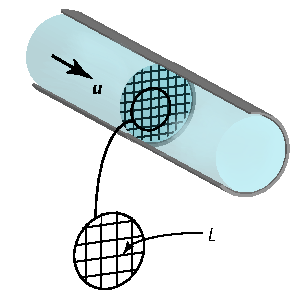
\includegraphics[width=\textwidth]{Figures/turbulence-maker}
\caption{\label{f.turbulence} A simple mechanism for generating turbulence. A flow of water in a pipe (upstream velocity $U$) flows through a mesh (spacing $L$).  If $\Rey = UL/\nu$ is sufficiently large, the downstream flow becomes turbulent. }
\end{figure}

\section{Exercises}
\begin{enumerate}
\item Assuming that $\nabla \approx \nabla_{\mathrm{ad}}$ in a convective region, sketch a plot of temperature as a function of pressure for the following cases.
\begin{enumerate}
\item A star with a stable inner layer and a convective outer layer;
\item A star with a convective inner layer and and a stable outer layer.
\end{enumerate}
Indicate on both of these plots an adiabat.
\end{enumerate}